\section{Phân tích phần dư và kỹ thuật làm trơn LOWESS}
\label{sec:4_2_residuals_lowess}

Phân tích phần dư (residual analysis) là phương pháp dùng để phát hiện sai lệch hệ thống chưa được mô hình mô tả. Phần dư (residuals) là chênh lệch đại số giữa giá trị quan trắc thực tế từ thiết bị cảm biến và giá trị tiên đoán từ phương trình lý thuyết. Đối với một hệ thống đo lường lý tưởng, ví dụ như bài toán rơi tự do nơi lực tác dụng duy nhất là trọng lực, phần dư của mô hình tọa độ được kỳ vọng sẽ phân bố ngẫu nhiên quanh trục hoành. Nếu phần dư xuất hiện xu hướng rõ ràng (systematic trend) trên đồ thị phân tán, điều đó phản ánh sự hiện diện của các hiệu ứng vật lý khác tác động lên đối tượng đo lường.

Thuật toán làm trơn LOWESS (Locally Weighted Scatterplot Smoothing) từ thư viện \texttt{statsmodels} được áp dụng để trực quan hóa các xu hướng phi tuyến này. Là một phương pháp hồi quy cục bộ phi tham số (non-parametric local regression), LOWESS tạo ra một đường cong liên tục biểu diễn xu hướng chính của phần dư mà không yêu cầu xác định trước bất kỳ cấu trúc hàm giải tích cụ thể nào.

\begin{pycode}{Residual analysis and non-parametric LOWESS smoothing}
import statsmodels.api as sm

# 2. Residual Analysis and Non-parametric LOWESS Smoothing
lowess_model = sm.nonparametric.lowess
smoothed_residuals = lowess_model(residuals_s, time_data, frac=0.4)

fig, ax = plt.subplots(figsize=(8, 5))
ax.scatter(time_data, residuals_s, color='black', edgecolor='black', alpha=0.6, label=r'$\mathrm{Algebraic \ Residuals}$')
ax.plot(smoothed_residuals[:, 0], smoothed_residuals[:, 1], 'r--', linewidth=2, label=r'$\mathrm{LOWESS \ Trend}$')
ax.axhline(0, color='blue', linestyle='--', linewidth=1.2)
ax.set_xlabel(r'$\mathrm{Time} \ t \ (\mathrm{s})$')
ax.set_ylabel(r'$\mathrm{Residuals} \ \Delta s \ (\mathrm{m})$')
ax.set_title(r'$\mathrm{Diagnostic \ Analysis: \ LOWESS \ Smoothing}$')
ax.legend()
ax.grid(True, linestyle=':', alpha=0.7)

plt.show()
\end{pycode}

\begin{figure}[htbp]
    \centering
    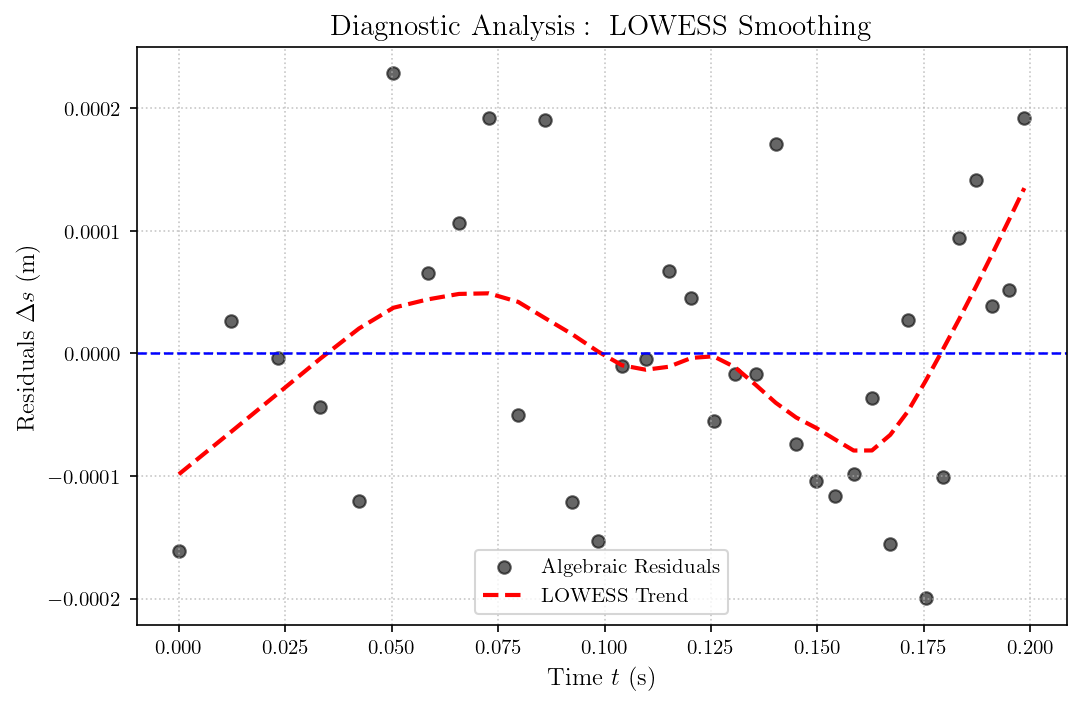
\includegraphics[width=\textwidth]{figures/fig_lowess_diagnostics.png}
    \caption{Phân tích phần dư và chẩn đoán xu hướng hệ thống thông qua kỹ thuật làm trơn LOWESS.}
    \label{fig:lowess_diagnostics}
\end{figure}

Khi áp dụng thuật toán làm trơn này lên chuỗi phần dư của dữ liệu tọa độ, đường cong LOWESS cung cấp cơ sở thống kê để đánh giá các điều kiện thực nghiệm phi lý tưởng.

\begin{physcore}{Đánh giá lực cản khí động học qua cấu trúc phần dư}{aerodynamic_drag}
Trong bài toán rơi tự do thực tế, nếu vật thể rơi trong môi trường không khí và có lực cản không khí đáng kể, phương trình lý thuyết sẽ không còn mô tả tốt dữ liệu. Lực cản không khí thường gia tăng theo bình phương vận tốc. Khi vật thể gia tốc theo thời gian, quãng đường thực tế có xu hướng chậm dần so với dự đoán từ hàm bậc hai. Sự sai lệch này làm phát sinh các giá trị phần dư âm ở giai đoạn cuối của quá trình thu thập dữ liệu. Việc đường LOWESS bẻ cong xuống dưới dải không (zero-line) tại các mốc thời gian lớn cho thấy để đánh giá mức độ tác động của lực cản khí động học (aerodynamic drag) đối với mô hình.
\end{physcore}

% \begin{pitfall}{Kiểm soát băng thông cục bộ trong thuật toán LOWESS}{lowess_bandwidth}
\begin{pitfall}{Ảnh hưởng của tham số phân số băng thông (frac) đến độ trơn LOWESS}{lowess_bandwidth}
Một vấn đề thường gặp khi sử dụng thuật toán LOWESS là việc cấu hình thiếu hợp lý tham số phân số băng thông (bandwidth fraction), được điều chỉnh thông qua đối số \texttt{frac}. Nếu \texttt{frac} quá nhỏ, mô hình sẽ gặp hiện tượng quá khớp (overfitting), khiến đường cong bị gãy khúc do bám sát các dao động ngẫu nhiên sinh ra từ giới hạn phân giải của thiết bị đo. Ngược lại, một giá trị \texttt{frac} tiệm cận $1.0$ sẽ gây ra hiện tượng phẳng hóa quá mức (oversmoothing), làm mờ đi đáng kể xu hướng tổng thể phản ánh các yếu tố vật lý (như lực cản không khí). Đối với các tập dữ liệu động học tự động hóa, việc thiết lập mức băng thông khoảng $\text{frac}=0.4$ thường cho kết quả ổn định, giúp đường cong LOWESS thể hiện rõ xu hướng chính mà không bị nhiễu cục bộ chi phối.
\end{pitfall}